% !TEX encoding = UTF-8 Unicode
% !TEX TS-program = pdflatex

%%%%%%% La riga soprastante serve per configurare gli editor
%%%%%%% TeXShop, TeXworks e TeXstudio per gestire questo file
%%%%%%% con la codifica UFF-8.
%%%%%%% Se si vuole usare un'altra codifica si veda sotto.
%%%%%%%

%%%%%%%  Esempio con molte opzioni
%%%%%%% Le opzioni nella forma "chiave=valore" sono definite
%%%%%%% perché la classe dalla versione 6.1.00 usa il pacchetto
%%%%%%% xkeyval. Vedere sulla documentazione in inglese o
%%%%%%% in italiano quali chiavi accettano valori.

%%%%%%% L'opzione per il corpo accetta qualsiasi valore, anche fratto
%%%%%%% (per esempio: corpo=11.5pt) e va sempre scritto con una
%%%%%%% unità di misura. L'utente è pregato di non esagerare con
%%%%%%% corpi normali minori di 9.5pt o maggiori di 13pt.
%%%%%%%
%%%%%%% Le opzioni per inputenc e fontenc vanno per prime.
%%%%%%% Vengono ignorate se NON si compone con pdfLaTeX. Ma
%%%%%%% questo è un esempio per pdfLaTeX.
%%%%%%%

 \documentclass[%
    corpo=12pt,
    twoside,
    stile=classica,   
% 	oldstyle,
%    autoretitolo,
    tipotesi=magistrale,
    greek,
    evenboxes,
    english
]{toptesi}
%%%%%%%%%%%%%%%%%%%%%%%%%%%%%%%%%%%%%%%%%%%%%%%%%%%%
%%%%%% Per la codifica d'entratasi può scegliere quella che si vuole,
%%%%%% ma si consiglia di preferire utf8; in ogni caso non scegliere
%%%%%% codifiche specifiche del sistema operativo.

\usepackage[utf8]{inputenc}% codifica d'entrata
\usepackage[T1]{fontenc}%    codifica dei font
\usepackage{lmodern}%        scelta dei font

% Vedere la documentazione toptesi-it.pdf per le
% attenzioni che bisogna usare al fine di ottenere un file
% veramente conforme alle norme per l'archiviabilità.


\usepackage[hidelinks]{hyperref}

\hypersetup{%
	pdfauthor={Gabriele Degola},
    pdfpagemode={UseOutlines},
    bookmarksopen,
    pdfnewwindow=true,
    pdfstartview={FitH}
  }
%
%%%%%%% Esempio di composizione di tesi di laurea con PDFLATEX 
%
\usepackage{lipsum}
\usepackage{subcaption}
\usepackage{biblatex}
\addbibresource{references.bib}
\usepackage[acronym]{glossaries}
%

\makeglossaries
\newacronym{ai}{AI}{artificial intelligence}
\newacronym{ilsvrc}{ILSVRC}{ImageNet Large Scale Visual Recognition Challenge}
\newacronym{cnn}{CNN}{Convolutional Neural Network}
\newacronym{svm}{SVM}{Support Vector Machines}
\newacronym{ide}{IDE}{Integrated Development Environment}
\newacronym{iou}{IoU}{Intersection over Union}
\newacronym{roc}{ROC}{Receiver Operating Characteristic}
\newacronym{auc}{AUC}{Area Under the Curve}
\newacronym{ap}{AP}{Average Precision}
\newacronym{map}{mAP}{mean Average Precision}
\newacronym{json}{JSON}{JavaScript Object Notation}
\newacronym{xml}{XML}{Extensible Markup Language}
\newacronym{voc}{VOC}{Visual Object Classes}
\newacronym{kitti}{KITTI}{Karlsruhe Institute of Technology and Toyota Technological Institute}
\newacronym{rcnn}{R-CNN}{region-based Convolutional Neural Network}
\newacronym[firstplural=Regions of Interest (RoIs)]{roi}{RoI}{Region of Interest}
\newacronym{rpn}{RPN}{Region Proposal Network}
\newacronym{fpn}{FPN}{Feature Pyramid Network}
\newacronym{ssd}{SSD}{Single Shot Detector}
\newacronym{yolo}{YOLO}{You Only Look Once}
\newacronym{adda}{ADDA}{Adversarial Discriminative Domain Adaptation}
\newacronym{dann}{DANN}{Domain Adversarial Neural Network}
\newacronym{coco}{COCO}{Common Objects in Context}
\newacronym[firstplural=GPUs]{gpu}{GPU}{Graphics Processing Unit}
\newacronym{cpu}{CPU}{Central Processing Unit}

\glsdisablehyper

%%%%%%% Definizioni locali
\newtheorem{osservazione}{Osservazione}% Standard LaTeX
\ExtendCaptions{english}{Abstract}{Acknowledgements}

\begin{document}\errorcontextlines=9
%%%%%%% Questi comandi è meglio metterli dentro l'ambiente
%%%%%%% ThesisTitlePage con o senza asterisco, oppure in un file di
%%%%%%% configurazione personale. Si veda la documentazione
%%%%%%% inglese o italiana.
%%%%%%% Comunque i presenti comandi servono per comporre la
%%%%%%% tesi con i moduli di estensione standard del pacchetto
%%%%%%% TOPtesi.

\english

\begin{ThesisTitlePage}*
\ateneo{Politecnico di Torino}% nome generico dell'Universita'
%\nomeateneo{Weiss Turm}% eventuale nome proprio dell'universita'
\logosede[4.5cm]{logopolito}% logo dell'universita'
\FacoltaDi{DIPARTIMENTO DI\space}% Etichetta della facolta'
\facolta{AUTOMATICA E INFORMATICA}% facolta'
%\Materia{Remote sensing}
\titolo{Domain Adaptation for Object Detection}% 
\sottotitolo{A data augmentation approach}% 
\CorsoDiLaureaIn{Master Degree in\space}
\corsodilaurea{Data Science and Engineering}% per la laurea
\TesiDiLaurea{Master Thesis}
\def\Candidato{Candidate}
\candidato{Gabriele \textsc{Degola}}% per tutti i percorsi 
\AdvisorName{Supervisor}
\relatore{prof.\ Paolo Garza}% per la laurea e/o il dottorato
%\tutoreaziendale{dott.\ ing.\ Giovanni Giacosa}
%\NomeTutoreAziendale{Supervisore aziendale\\Centro Ricerche FIAT}

\sedutadilaurea{\textsc{Anno~accademico} 2021-2022}% per la laurea magistrale
\end{ThesisTitlePage}

\sommario



% \paginavuota % funziona anche senza specificare l'opzione classica

\ringraziamenti



\tablespagetrue\figurespagetrue % normalmente questa riga non serve ed e' commentata
\indici

\mainmatter

\chapter*{Introduction}

\chapter{Problem definition}

\section{Object detection}
Object detection methods are able to recognize the objects represented in an image and to highlight their position, returning the associated bounding boxes, rectangular boxes which contain an object. The bounding box format depends on the model and on the dataset. Typically, they are determined by the \textit{x} and \textit{y} coordinates of the upper-left corner
%, as in \acrshort{coco} (\ref{sec:coco}),
or of the center
%, as in \acrshort{yolo} (\ref{sec:yolo}),
and by the bounding box width and height.

\begin{figure}[ht]
	\centering
	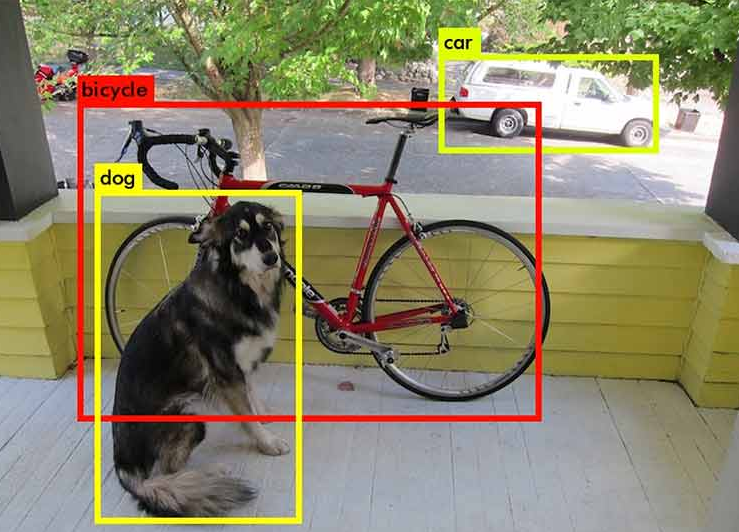
\includegraphics[width=.5\textwidth]{imgs/yolo_detection.png}
	\caption{An example of object detection\cite{redmon2016look}}
\end{figure}

Object detection is a fundamental task in modern computer vision, with applications such as autonomous driving, robot vision and human-computer interaction.

\subsection{Existing methods}
An object detection task can be seen as a combination of two main steps: finding image regions that may contain objects, and then independently classifying the objects in those regions. Before deep learning, this was achieved using a sliding-window approach, where an image classifier was applied to different areas of the image and only the predictions with the highest probability were retained. Nowadays, two main families of object detectors can be identified.

\subsubsection{Two stage object detectors}
As said, the most commonly used models for object detection are based on a two-stage approach and belong to the family of \glspl{rcnn}. In basic \acrshort{rcnn}\cite{girshick2014rich}, a manageable number of possible \glspl{roi} are extracted from an image and a \gls{cnn} is evaluated independently on each \acrshort{roi} to extract features that are fed into a \gls{svm} to classify the presence of an object in that region and the bounding box location. Fast \acrshort{rcnn}\cite{girshick2015fast} and Faster \acrshort{rcnn}\cite{ren2016faster} improved the region selection algorithm, analysing only interesting \glspl{roi} and exponentially reducing the inference time. Because of its good performances and speed, Faster \acrshort{rcnn} is widely used for benchmarking and as base for several derived works.


The main contribution of Faster \acrshort{rcnn} is the introduction of a \gls{rpn}, which integrate some convolutional layers of the image classifier into the region proposal phase. That allows the network to be trained in an end-to-end fashion.

\begin{figure}[ht]
	\centering
	\subcaptionbox{Description of \acrshort{rcnn}\cite{girshick2014rich}}{
		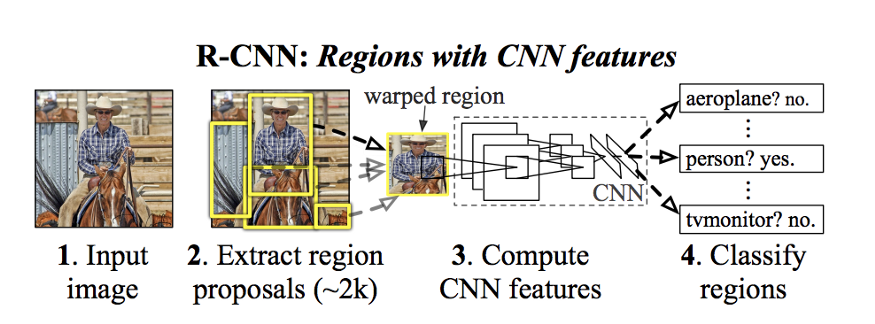
\includegraphics[width=.6\linewidth]{imgs/rcnn.png}
	}
	\subcaptionbox{Description of Faster \acrshort{rcnn}\cite{ren2016faster}}{
		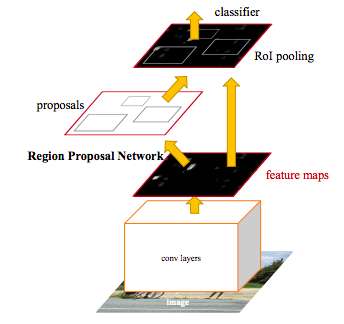
\includegraphics[width=.3\linewidth]{imgs/fasterrcnn.png}
	}
	\caption{Architecture of two stage object detectors}
	\label{fig:architectures}
\end{figure}

\subsubsection{One stage object detectors}
Differently from two stage detectors, one stage object detectors skip the region proposal step and focus on predicting object regions and classes together. This leads to faster predictions with respect to two stage models, making them suitable for real-time applications at the cost of lower prediction quality. The pioneer work for one stage object detection is OverFeat\cite{sermanet2014overfeat}, published in 2014. Here, the last classification layers of a standard \gls{cnn} are replaced by a regression network for each class, in order to predict the object bounding boxes.

\paragraph{YOLO}\label{sec:yolo}
The \acrfull{yolo} model\cite{redmon2016look} uses pretrained \gls{cnn} for classification and splits each image in cells. If the center of an object falls into a cell, that cell is responsible for detection and should predict the bounding box locations, a confidence score and a class probability for the detected objects. A specific loss function is used to efficiently learn at the same time to predict bounding boxes and object classes.

\paragraph{SSD}
\acrfull{ssd}\cite{Liu_2016} adds several convolutional layers of decreasing sizes, in order to build a \textit{pyramid representation} of the images and efficiently detect object of different sizes, at each pyramidal layer. Instead of splitting images in cells, anchor boxes are used for faster detection.

\begin{figure}
	\centering
	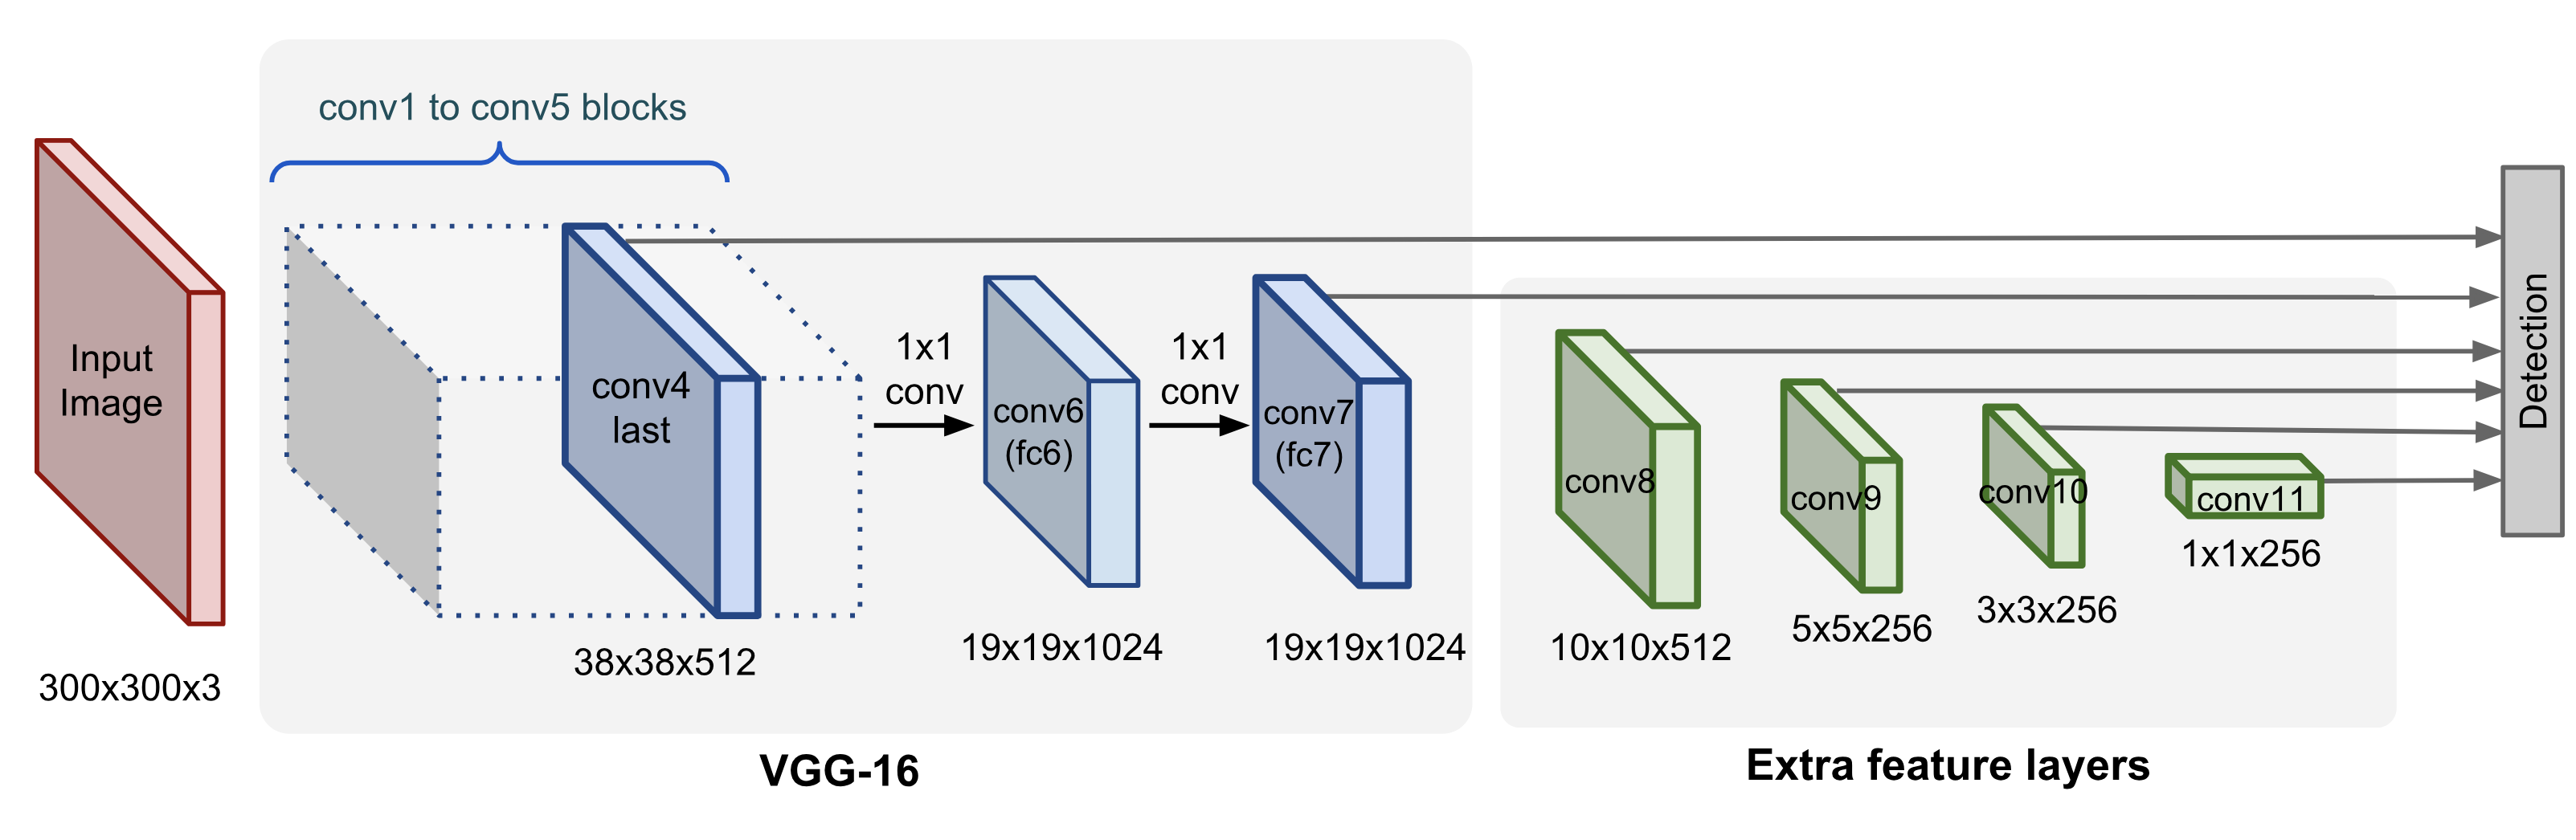
\includegraphics[width=.7\linewidth]{imgs/SSD-architecture.png}
	\caption{\acrshort{ssd}'s pyramid architecture\cite{objdetpart4}}
	\label{fig:ssd}
\end{figure}

\paragraph{RetinaNet}
The main improvements of RetinaNet\cite{lin2018focal} over previous one stage detection model are the use of \textit{feature pyramid network} as part of the backbone and of \textit{focal loss}, which helps to approach the results of two-stage detectors.

\begin{figure}[ht!]
	\centering
	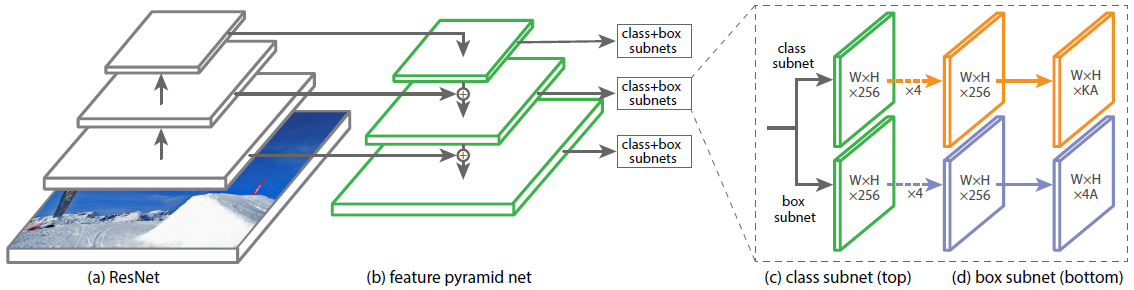
\includegraphics[width=0.8\linewidth]{imgs/retinanet.png}
	\caption{RetinaNet architecture\cite{lin2018focal}}
	\label{fig:retinanet}
\end{figure}

\subparagraph{Feature pyramid network}
\glspl{fpn}\cite{lin2017feature} adopt and improve the same approach as \acrshort{ssd}'s pyramid layers. They are composed by a sequence of pyramid levels which correspond to network stages. Each stage is composed by multiple convolutional layers of the same size, divided by two at consecutive stages. In addition to standard feedforward, different stages are linked by a top-down pathway in the opposite direction and lateral connections. This allows the network to construct a rich and multi-scale feature pyramid for each input image.

After their proposal in the context of single-stage detectors, the \glspl{fpn} have also been used as part of the backbone of two-stage detectors, to improve their performance.

\subparagraph{Focal loss}
One of the main obstacles for the training of  other object detector models is the large imbalance between background and foreground examples, which drives the model to focus on irrelevant background regions.

The focal loss, introduced by RetinaNet, is based on the \textit{cross entropy} loss. For binary classification, the cross entropy loss is widely used and defined as:
\begin{center}
	$CE(p,y) = \begin{cases}
		-\log(p) & \text{if $y$ = 1}\\
		-\log(1-p) & \text{otherwise.}
	\end{cases}$
\end{center}
where $y\in \{\pm 1\}$ is the ground truth class and $p\in\left[0,1\right]$ is the model's probability for class $1$. Defining $p_t$ as:
\begin{center}
	$p_t = \begin{cases}
		p & \text{if $y$ = 1}\\
		1-p & \text{otherwise.}
	\end{cases}$
\end{center}
cross entropy can be written as $CE(p,y) = CE(p_t) = -\log(p_t)$.

\bigskip
A balanced version of the cross entropy loss is sometimes used to deal with class imbalance. A numeric factor $\alpha\in\left[0,1\right]$ can be introduced for class $1$, with value $1-\alpha$ for class $-1$. $\alpha_t$ is defined analogously to $p_t$. Therefore, the balanced cross entropy is written as:
\begin{center}
	$CE(p,y) = -\alpha_t\log(p_t)$.
\end{center}

\bigskip
With cross entropy, also easily classified example ($p$ close to $1$ if $y=1$, to $0$ otherwise) produce a non-negligible value for the loss. In focal loss, an additional modulating factor $\left(1-p_t\right)^\gamma$ is added, with tunable focusing parameter $\gamma$. Focal loss is therefore defines as:
\begin{center}
	$FL(p_t) = -\left(1-p_t\right)^\gamma \log(p_t)$
\end{center}
The contribution of easy detections to the overall loss is more or less important depending on the value of $\gamma$. With a high $\gamma$, well detected objects provide a very little contribution to the total loss.

Considering the strong imbalance between the foreground ($y=1$) and background ($y=-1$) classes, the focal loss balanced by the $\alpha_t$ parameter as previously defined is used in RetinaNet:
\begin{center}
	$FL(p_t) = -\alpha_t\left(1-p_t\right)^\gamma \log(p_t)$.
\end{center}

\subsection{Basic components}
\subsubsection{Metrics}
Algorithm evaluation is a fundamental part of machine learning projects and can be performed in different ways, depending on the task and objective. Object detection is a more complex task than traditional classification: a non-fixed number of objects can be present in the same image and the detection model has to accurately predict their position and class. For this reason, dedicated metrics must be introduced and defined.

\paragraph{Precision and recall}
First, the following concepts must be defined in the context of object detection:
\begin{itemize}
	\item \textbf{True positive} (TP): object correctly detected;
	\item \textbf{False positive} (FP): incorrect detection, an object is detected but is not actually present in the bounding box or only partly;
	\item \textbf{False negative} (FN): an object present is the image is not detected by the model.
\end{itemize}
The concept of true negative (TN) does not make sense in an object detection context, as the missing detection of a non-present object is not relevant. In fact, this would mean that the model has correctly identified the background as not belonging to any class.

\subparagraph{Precision}
Precision measures how accurate the predictions of the model are, so it returns the percentage or fraction of correct prediction.
\begin{center}
	$precision = \frac{TP}{TP+FP}$
\end{center}

\subparagraph{Recall}
Recall measures the model detection ability, so it returns the percentage or fraction of correctly detected objects.
\begin{center}
	$recall = \frac{TP}{TP+FN}$
\end{center}

\paragraph{Intersection over union}
For each predicted bounding box, the overlapping with the ground truth bounding boxes is computed, in order to classify the prediction as true or false positive. For a couple of bounding boxes, it is computed as:
\begin{center}
	$IoU = \frac{area\ of\ overlap}{area\ of\ union}$
\end{center}
The computed value is then compared to a threshold to classify a prediction as correct or not. Typical values for the threshold are $0.5$, $0.75$ and $0.95$ and that defines how much we want a detection to be precise. Indeed, a detection classified as true positive with a certain threshold may be considered as false positive if a higher value is used.

\paragraph{Mean Average Precision (mAP)}
\gls{roc} curve is a popular concept in machine learning. There, recall (or true positive rate) and false positive rate are plotted at different classification thresholds. The associated \gls{auc} metric considers the area under the \gls{roc} curve to assess the performances of a model.\cite{roc} It ranges from $ 0 $ to $ 1 $, with $ 0 $ meaning the model's predictions are all wrong and $ 1 $ they are all correct. Ideally, the \gls{auc} score is $ 0.5 $ for a model that returns random predictions.

Similarly, the precision-recall curve shows the trade-off between precision and recall for different thresholds\cite{precrecall}. \gls{ap} is defined as the area under the precision-recall curve. A high area under the curve means both high recall and high precision. The definition of \gls{map} depends on the context. If \gls{ap} is independently computed for each class or for different \gls{iou} thresholds, then \gls{map} is the average of \gls{ap}. In other cases, \gls{map} and \gls{ap} can be used interchangeably.


\subsubsection{Datasets}\label{sec:datasets}
Several datasets have been published to evaluate the performances of object detection algorithms for different use cases.

\paragraph{COCO}\label{sec:coco}
\acrfull{coco} is a large-scale object detection and object segmentation dataset published by Microsoft, containing over 200000 images for 91 classes, annotated with bounding boxes and at pixel level\cite{lin2015microsoft}. It defines its own annotation format as \acrshort{json} files.

\paragraph{PASCAL VOC}
PASCAL \acrfull{voc} is a classification and object detection dataset, developed for different machine learning competitions between 2005 and 2012\cite{voc}. Annotations are stored in \acrshort{xml} format, with a file for each image in the dataset. Bounding boxes are determined by the $x$ and $y$ coordinates of the upper left and bottom left corners.

\paragraph{CityScapes}
CityScapes is an object segmentation dataset containing 5000 street scenes images from 50 different cities, with the aim of training models for autonomous driving\cite{cordts2016cityscapes}. When used for object detection, bounding boxes can be derived from the tightest rectangles containing the segmentation masks.

\paragraph{KITTI}
The \acrfull{kitti} dataset\cite{Geiger2013IJRR} contains 7481 images captured in a context similar to CityScapes. Bounding box annotations are stored in plain text, with one file per image.

\paragraph{Sim10k}
Sim10k is a synthetic dataset containing 10000 annotated images for car detection, rendered from the video-game Grand Theft Auto 5, with the objective of training models in a rich virtual world for detection in the real\cite{johnsonroberson2017driving}.

\begin{figure}[ht]
	\centering
	\subcaptionbox{CityScapes\cite{cordts2016cityscapes}}{
		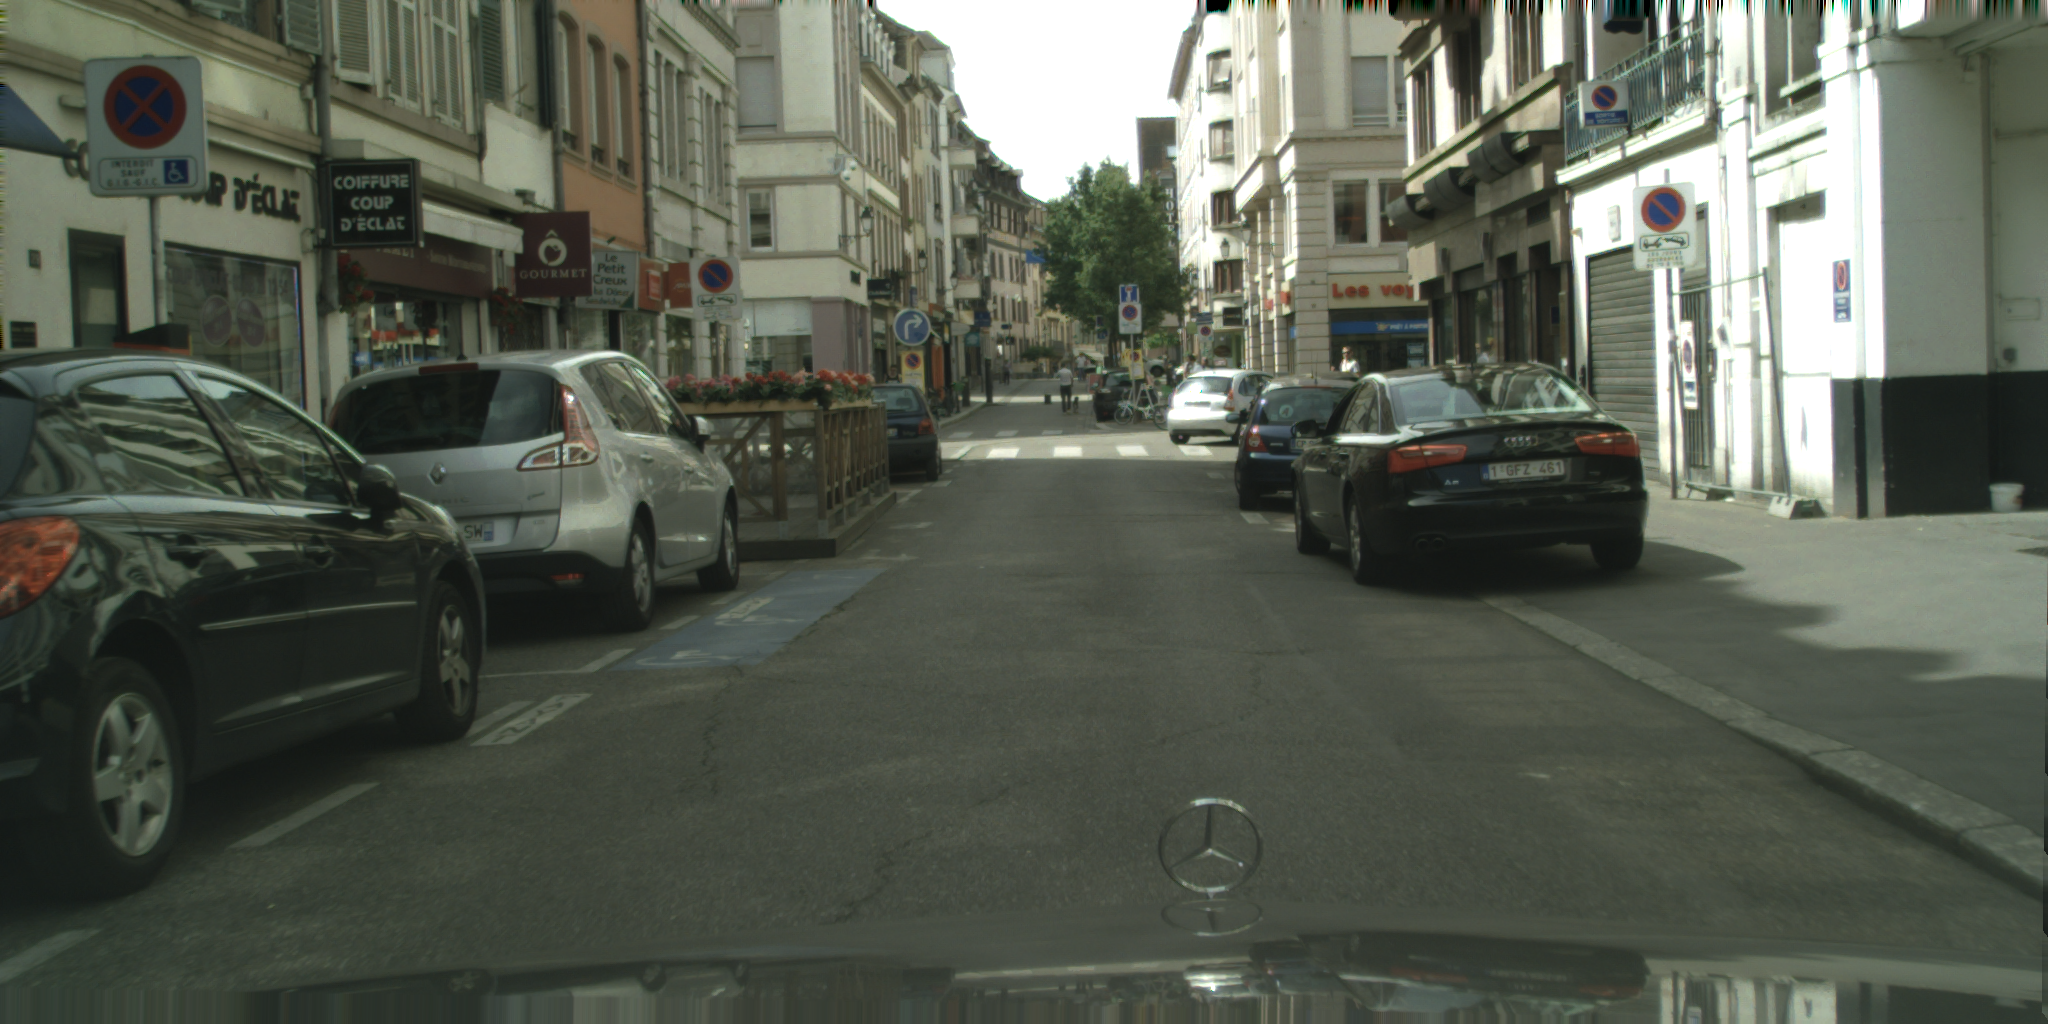
\includegraphics[width=.3\linewidth]{imgs/cityscapes.png}
	}
	\subcaptionbox{\acrshort{kitti}\cite{Geiger2013IJRR}}{
		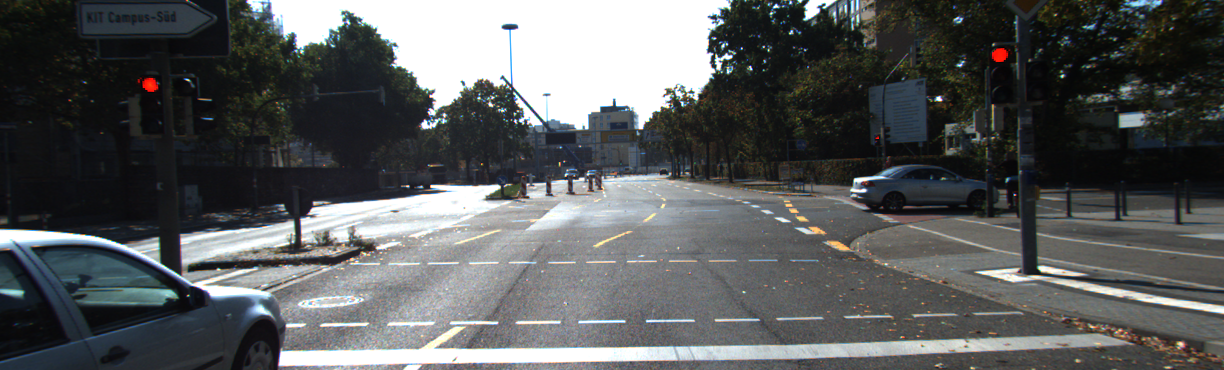
\includegraphics[width=.31\linewidth]{imgs/kitti.png}
	}
	\subcaptionbox{Sim10k\cite{johnsonroberson2017driving}}{
		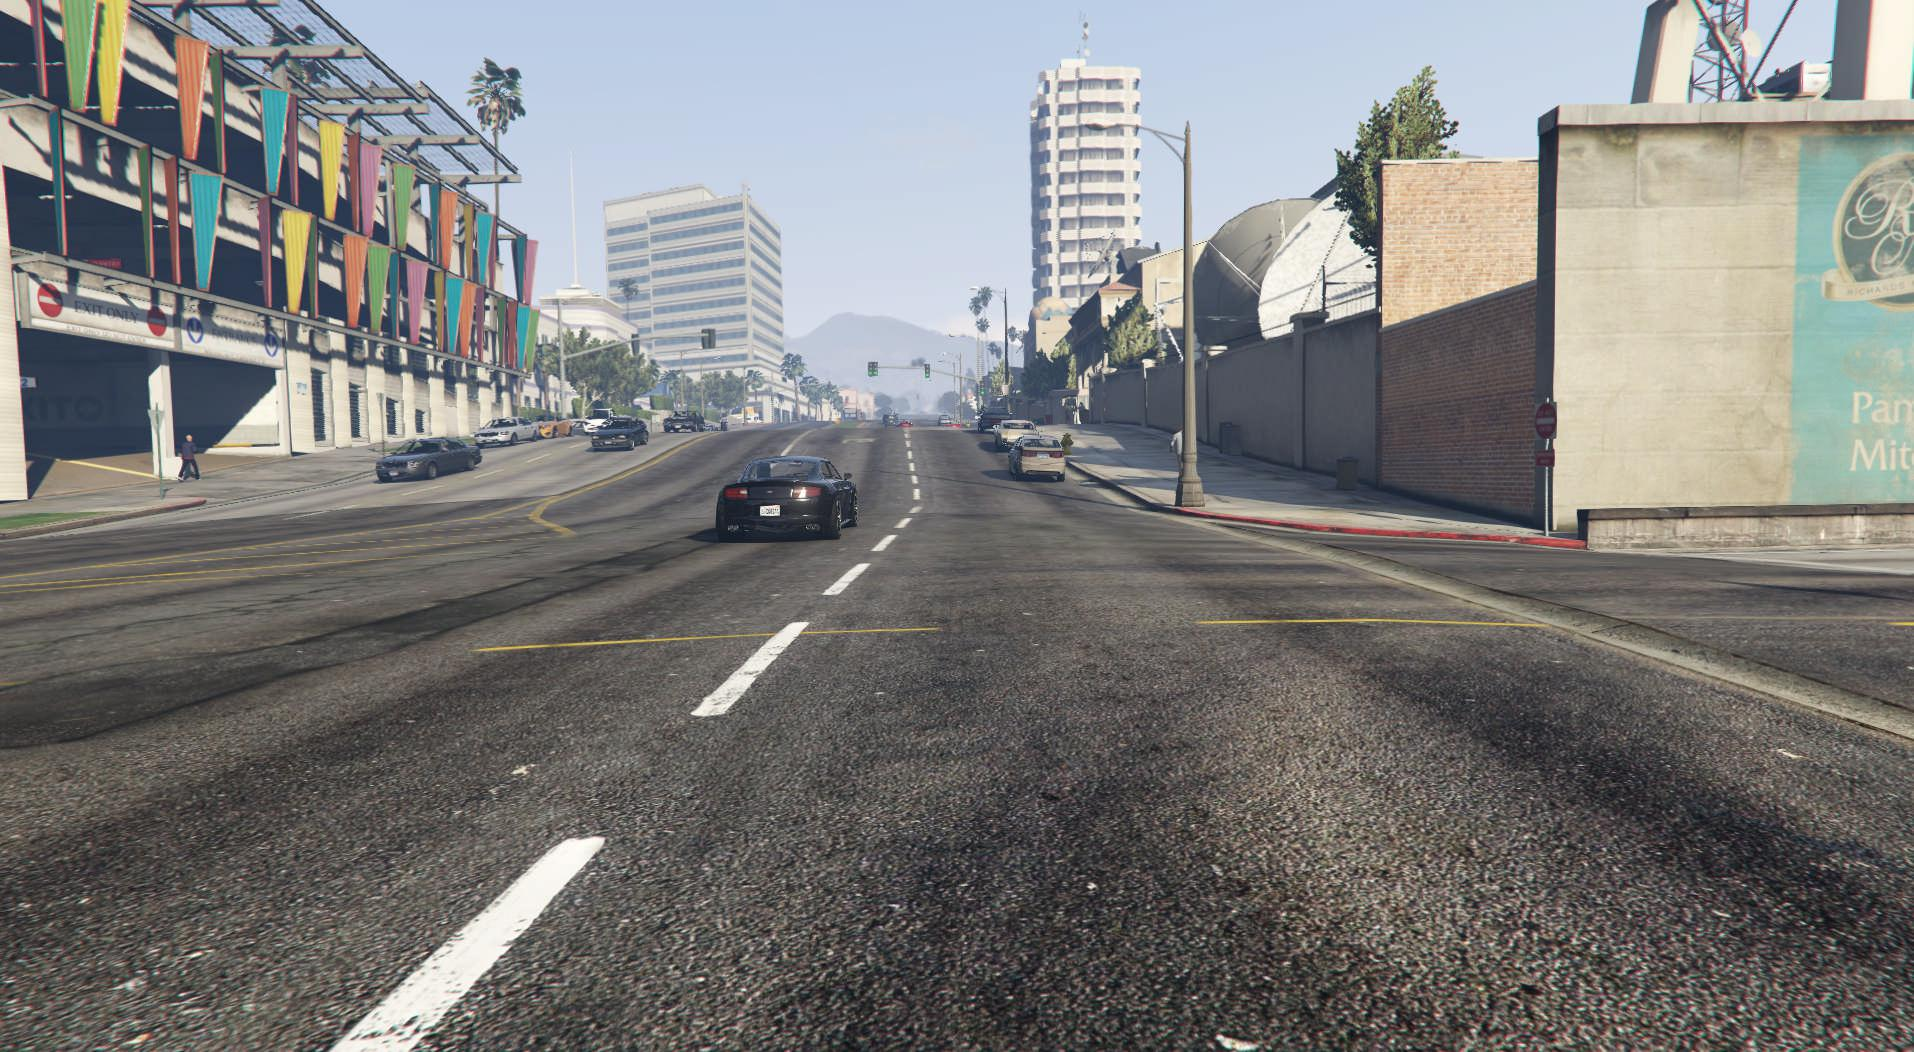
\includegraphics[width=.31\linewidth]{imgs/sim10k.jpg}
	}
	\caption{Examples of different street scenes datasets. It is evident that the appearance of images from different domains varies, even if they contain the same categories of objects.}
	\label{fig:datasets}
\end{figure}

\subsubsection{Anchor boxes}\label{sec:anchor}
In most cases, generating a large number of possible bounding boxes is too cumbersome and leads to inaccurate predictions. If we already know which classes we want to detect, it may be more efficient to define a-priori a set of possible aspect ratios and zoom factors for the bounding boxes. For example, if we are interested in detecting cars wide anchor boxes can be defined at different scales, to identify both near and far objects.

\subsubsection{Non-maximum suppression}
Object detection models usually produce more than one detection for each object, which is not desirable. Non-maximum suppression (NMS) is a method to select one of many overlapping bounding boxes. For a set of overlapping boxes, the one predicted with the highest confidence is selected and all remaining boxes with \gls{iou} over a certain threshold are discarded.


\section{Domain adaptation}
For most cases, a huge number of annotated images are necessary to train robust and efficient deep learning models. In an industrial context, the process of collecting and annotating data suitable for each specific customer case is often too expensive and time-consuming. In contrast, synthetic data can be generated through various rendering softwares, even free and open-source, easily and in massive quantities, for simulating the environments in which the models will be applied. However, deep learning models are effective if the training and test data are drawn from the same distribution, so a model trained on simulated data is likely to perform badly on real data. Domain adaptation techniques can be used to transfer knowledge acquired on the \textbf{source domain} (e.g., synthetic data) to the \textbf{target domain} (e.g., real data) without training a new model on the latter. In a domain adaptation setting, the task to be performed on source and target domains and the classes to be predicted remain the same, while the domain differs.
% elencare altri casi di DA

%\blankpagestyle{headings}

%\lipsum[1-2]

\chapter{Method}

\chapter{Experiments and results}

\chapter*{Conclusions}

\backmatter
\printbibliography[heading=bibintoc]


\end{document}
